%
% Example file
%

\documentclass{fose2019}           % for pLaTeX2e
%\documentclass[english]{fose2016} % for English papers
%\documentclass[ascii]{fose2016}   % for ASCII pTeX

\usepackage[dvipdfmx]{graphicx}
%\usepackage{epsfig}

\title{fose2019.cls 使用サンプル}
\etitle{An example of use for fose2019.cls}
\journalhead{An example of use for fose2019.cls}
\author{磯崎 秀樹}{Hideki Isozaki, NTT基礎研究所}
\author{徳川 家康}{Ieyasu Tokugawa, 江戸幕府}

\begin{document}

\maketitle


\begin{abstract}
これは,{\tt fose2019.cls}スタイルファイルを利用し,
\LaTeX でフォーマットしたFOSE2019の論文サンプルです.
\begin{itemize}
\item 論文本文が和文の場合,和文・英文のいずれかでアブストラクトを
書いて下さい.両方併記することもできます.英文アブストラクトを書く
場合は{\tt eabstract}環境(\verb|\begin{eabstract}?\end{eabstract}|)を
使って下さい.
\item 本文が英文の場合は,{\verb|\documentclass[english]{fose2019}|}コマンドを利用して下さい.
また,和文タイトル・和文著者名・和文アブストラクトを併記する必要はありません.
\end{itemize}
\end{abstract}
\begin{eabstract}
This document has been prepared as a sample for typesetting
FOSE2019 papers using the FOSE2019 \LaTeX \ style file.
\end{eabstract}

\section{ワークショップの目的}
情報技術の普及がソフトウェアの適用範囲をますます広げていく今,ソフトウェアを社会基盤となる知的資産として活用するため,ソフトウェア工学はさらに格段の進歩をとげなければなりません.FOSEはこの挑戦に向けてさまざまな基礎技術を確立することをめざし,研究者・技術者の議論の場を提供するものです.

\section{ワークショップ開催概要}
FOSE2019\cite{fose2019}は以下の要領で開催する予定です.
\begin{description}
\item[日程] 2019年11月15日(木) -- 17日(土)
\item[場所] 湯の川温泉 花びしホテル\\
{\footnotesize
   〒042--0932 北海道函館市湯川町1--16--18
}
\item[主催] 日本ソフトウェア科学会 ソフトウェア工学の基礎研究会
\item[共催] IEEE Computer Society Japan Chapter
\item[協賛] 情報処理学会 ソフトウェア工学研究会,\\
	電子情報通信学会 ソフトウェアサイエンス研究会,\\
	電子情報通信学会 知能ソフトウェア工学研究会
\end{description}

\section{書式に関して}
\subsection{ヘッダとフッタ}
カバーページを除く奇数ページのヘッダには,英語論文タイトルが来ます.
英語タイトルが長すぎたり,
任意の位置で改行したい場合には\verb|\journalhead{The Title}|を利用して下さい.
偶数ページのヘッダには「FOSE2019」が来ます.
フッタは空となるように設定してください.

\subsection{箇条書き}
\begin{itemize}
\item 項目1
\item 項目2
  \begin{itemize}
  \item 項目2-1
  \item 項目2-2
  \end{itemize}
\end{itemize}

\begin{enumerate}
\item 項目3 (項番付き)
  \begin{enumerate}
  \item 項目3-1 (項番付き)
  \item 項目3-2 (項番付き)
  \end{enumerate}
\end{enumerate}

\subsection{表と図}

表の例を表\ref{tab:example}に,
図の例を図\ref{fig:example}に示します.

\begin{table}[htbp]
  \centering
  \caption{表の例} \label{tab:example}
  \begin{tabular}{|l|l|l|}\hline
%    FOSE2001 & ソフトウェア工学の基礎 VIII & 杉山 安洋,藤田ハミド 編 \\ \hline
%    FOSE2002 & ソフトウェア工学の基礎 IX & 井上 克郎 編 \\ \hline
%    FOSE2003 & ソフトウェア工学の基礎 X & 鰺坂 恒夫,満田 成紀 編 \\ \hline
%    FOSE2004 & ソフトウェア工学の基礎 XI & 野呂 昌満,山本 晋一郎 編 \\ \hline
%    FOSE2005 & ソフトウェア工学の基礎 XII & 権藤 克彦,小林 隆志 編 \\ \hline
%    FOSE2006 & ソフトウェア工学の基礎 XIII & 沢田 篤史,丸山 勝久 編 \\ \hline
%    FOSE2007 & ソフトウェア工学の基礎 XIV & 岸 知二,野田 夏子 編 \\ \hline
%    FOSE2008 & ソフトウェア工学の基礎 XV & 松下 誠,川口 真司 編 \\ \hline
%    FOSE2010 & ソフトウェア工学の基礎 XVII & 高田 眞吾,福田 浩章 編 \\ \hline
%    FOSE2011 & ソフトウェア工学の基礎 XVIII & 門田 暁人,上野 秀剛 編 \\ \hline
%    FOSE2012 & ソフトウェア工学の基礎 XIX & 鵜林 尚靖,亀井 靖高 編 \\ \hline
    FOSE2013 & ソフトウェア工学の基礎 XX & 岡野 浩三,関澤 俊弦 編 \\ \hline
    FOSE2014 & ソフトウェア工学の基礎 XXI& 花川 典子,尾花 将輝 編\\ \hline
    FOSE2015 & ソフトウェア工学の基礎XXII & 青木 利晃,豊島 真澄 編\\ \hline
    FOSE2016 & ソフトウェア工学の基礎XXIII & 阿萬 裕久,横川 智教 編\\ \hline
    FOSE2017 & ソフトウェア工学の基礎XXIV & 吉田 敦,福安 直樹 編\\ \hline
    FOSE2018 & ソフトウェア工学の基礎XXV & 伊藤 恵,神谷 年洋  編\\ \hline
  \end{tabular}
\end{table}

\begin{figure}[htbp]
  \centering
  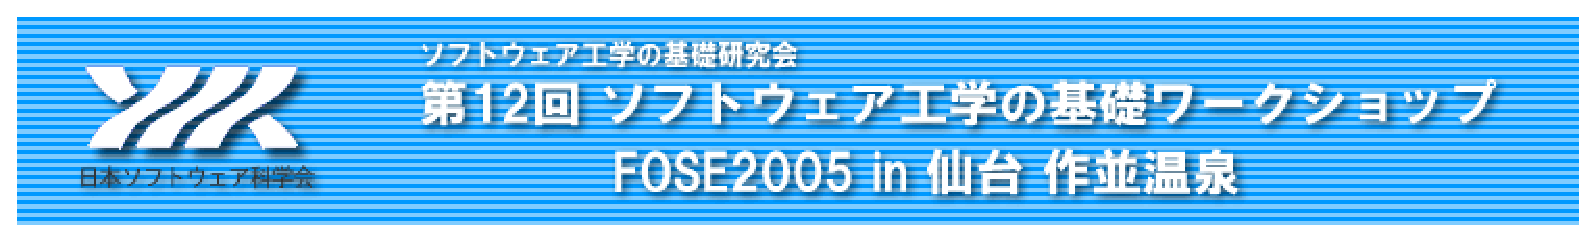
\includegraphics[width=\textwidth]{fose2005logo.eps}
%  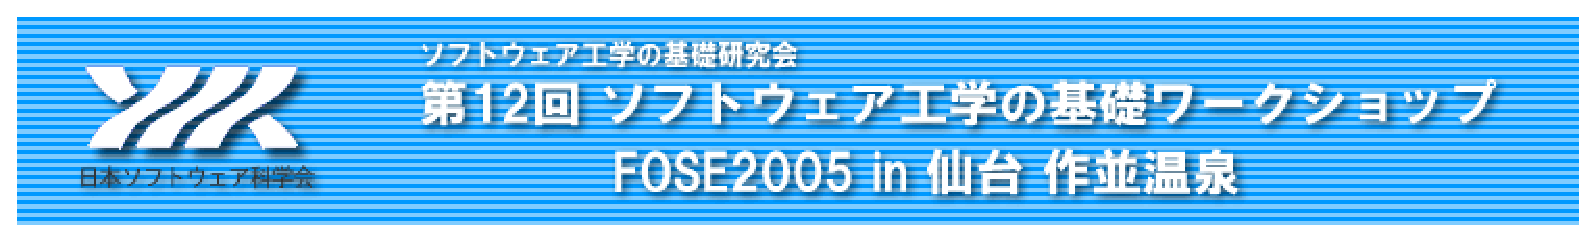
\epsfig{file=fose2005logo.eps,width=\textwidth}
  \caption{図の例(FOSE2005のロゴを使わせてもらっております)}
  \label{fig:example}
\end{figure}



\acknowledgements{}
本フォーマットを作成して頂いた方々に感謝します.
%また, \LaTeX2e 用のフォーマットを作成して頂ける方がいらっしゃいましたら,プログラム委員長までご連絡ください.

%\bibliography{own,related,misc}
\bibliographystyle{junsrt}

\begin{thebibliography}{9}
% \bibitem{fose2001} 杉山 安洋, 藤田 ハミド 編: ソフトウェア工学の基礎VIII,
%         日本ソフトウェア科学会{\em FOSE2001}, 近代科学社, 2001.
% \bibitem{fose2002} 井上 克郎 編: ソフトウェア工学の基礎IX,
%         日本ソフトウェア科学会{\em FOSE2002}, 近代科学社, 2002.
% \bibitem{fose2003} 鰺坂 恒夫, 満田 成紀 編:ソフトウェア工学の基礎X,
%         日本ソフトウェア科学会{\em FOSE2003}, 近代科学社, 2003.
% \bibitem{fose2004}野呂 昌満,  山本 晋一郎 編:ソフトウェア工学の基礎XI,
%         日本ソフトウェア科学会{\em FOSE2004}, 近代科学社, 2004.
% \bibitem{fose2005}権藤 克彦,  小林 隆志 編:ソフトウェア工学の基礎XII,
%         日本ソフトウェア科学会{\em FOSE2005}, 近代科学社, 2005.
% \bibitem{fose2006}沢田 篤史,  丸山 勝久 編:ソフトウェア工学の基礎XIII,
%         日本ソフトウェア科学会{\em FOSE2006}, 近代科学社, 2006.
% \bibitem{fose2007}岸 知二,野田 夏子 編:ソフトウェア工学の基礎XIV,
%         日本ソフトウェア科学会{\em FOSE2007}, 近代科学社, 2007.
% \bibitem{fose2008}松下 誠,川口 真司 編:ソフトウェア工学の基礎XV,
%         日本ソフトウェア科学会{\em FOSE2008}, 近代科学社, 2008.
% \bibitem{fose2009} 第16回ソフトウェア工学の基礎ワークショップ,
%         {\em http://www.washi.cs.waseda.ac.jp/fose2009/}, 2009.
% \bibitem{fose2010}高田 眞吾,福田 浩章 編:ソフトウェア工学の基礎XVII,
%         日本ソフトウェア科学会{\em FOSE2010}, 近代科学社, 2010.
% \bibitem{fose2011}門田 暁人,上野 秀剛 編:ソフトウェア工学の基礎XVIII,
%         日本ソフトウェア科学会{\em FOSE2011}, 近代科学社, 2011.
 \bibitem{fose2012}鵜林 尚靖,亀井 靖高 編:ソフトウェア工学の基礎XIX,
         日本ソフトウェア科学会{\em FOSE2012}, 近代科学社, 2012.
 \bibitem{fose2013}岡野 浩三,関澤 俊弦 編:ソフトウェア工学の基礎XX,
         日本ソフトウェア科学会{\em FOSE2013}, 近代科学社, 2013.
 \bibitem{fose2014}花川 典子,尾花 将輝 編:ソフトウェア工学の基礎XXI,
         日本ソフトウェア科学会{\em FOSE2014}, 近代科学社, 2014.
 \bibitem{fose2015} 青木 利晃,豊島 真澄 編:ソフトウェア工学の基礎XXII,
         日本ソフトウェア科学会{\em FOSE2015}, 近代科学社, 2015.
 \bibitem{fose2016} 阿萬 裕久,横川 智教 編:ソフトウェア工学の基礎XXIII,
	 日本ソフトウェア科学会{\em FOSE2016}, 近代科学社, 2016.
\bibitem{fose2017} 吉田 敦,福安 直樹 編:ソフトウェア工学の基礎XXIV,
	 日本ソフトウェア科学会{\em FOSE2017}, 近代科学社, 2017.
\bibitem{fose2018} 伊藤 恵,神谷 年洋 編:ソフトウェア工学の基礎XXV,
	 日本ソフトウェア科学会{\em FOSE2019}, 近代科学社, 2018. 
\bibitem{fose2019} 伊藤 恵,神谷 年洋 編:ソフトウェア工学の基礎XXVI,
	 日本ソフトウェア科学会{\em FOSE2019}, 近代科学社, 2019. (to appear)
\end{thebibliography}
\end{document}
